\section{DAPHNE Interfaces}
\label{sec:interfaces}

The FEB has a direct connection with 4 subsystems: Cold Electronics, DAQ, Slow control and timing interface.

\subsection{Cold electronics}

The front-end-board DAPHNE and the so called Cold Electronics (CE) are intended to work together in order to detect and process photons collected by the X-ARAPUCA system. The CE consist of SiPM arrays and amplification electronics that are powered by the DAPHNE board.  

Each array consists of 48 SiPMs, where groups of 6 SiPMs are connected in parallel and 8 groups are ganged together, so in essences the 48 SiPMs are connected in parallel and constitutes an analog channel. The signals  are preconditioned using the so called cold amplifier which drives signals over a 100 $\Omega$  differential pair. The differential treatment of the signal between the cold electronics and DAPHNE is mandatory for the signal integrity. The constraints for this treatment are the distance to the cryostat, the impedance of the carrier cables and the frequency of the expected pulses. 
 
 DAPHNE is responsible for providing the bias voltage for the SiPM and a digitally controlled trim voltage to the cold electronics. Another digital voltage is used as a reference for the analog signal conversion, that voltage reference moves the reference into the AFE. All these signals are driven by DACs attached to the FPGA. 


\subsubsection{Bias voltage}

DAPHNE supplies a bias voltage (56V) to SiPMs arrays. The bias voltage is generated from a HV output of the power supply circuit; the voltage value is set by soldering a bridge on the specific point on the board. The figure~\ref{fig:DACsStage} shows the general scheme for the voltages generation (bias, trimming and offset). 

\begin{figure}[htbp]
\centering % \begin{center}/\end{center} takes some additional vertical space
%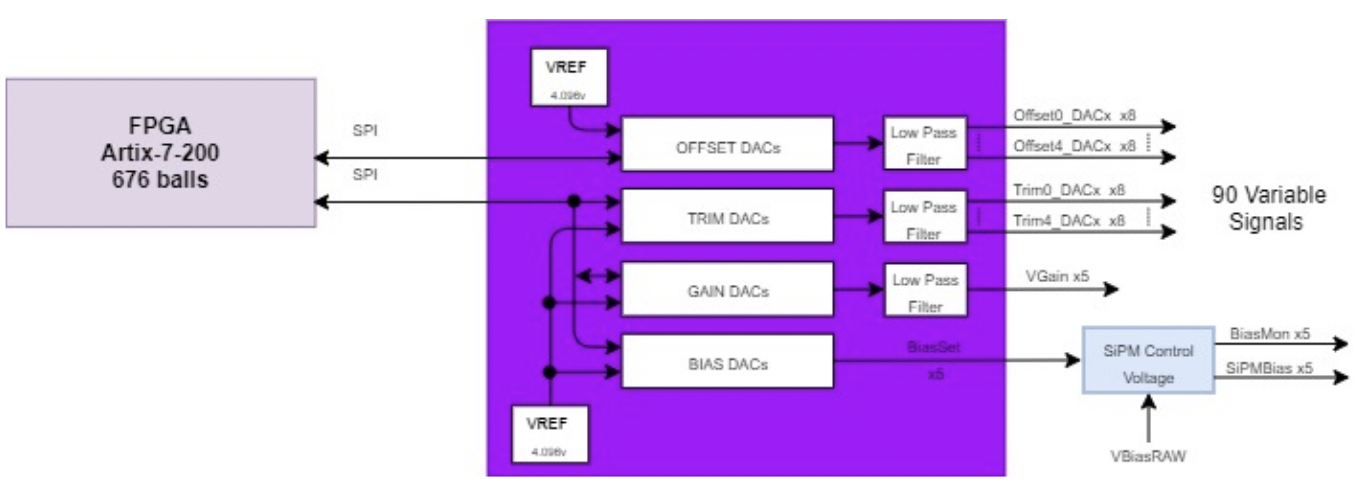
\includegraphics[width=.8\textwidth,trim=30 110 0 0,clip]{Images/BiasControl.png}
%\qquad
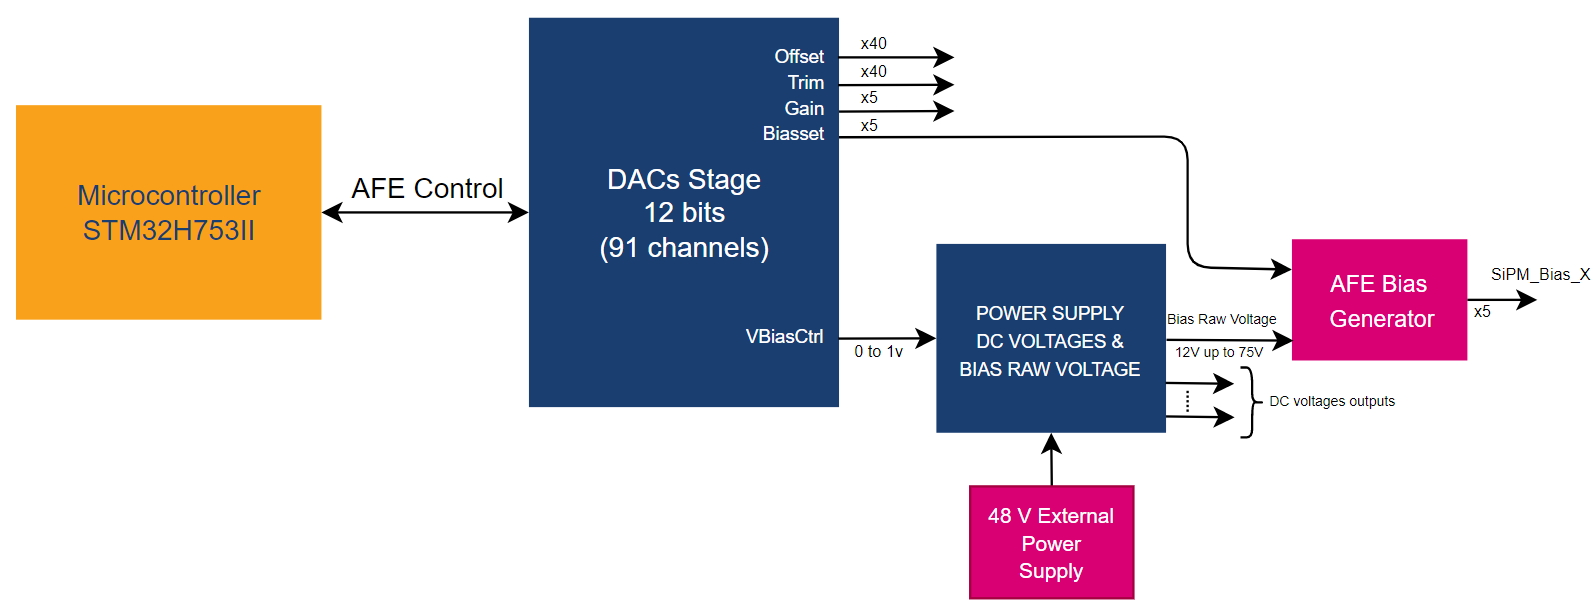
\includegraphics[width=.8\textwidth,origin=c,angle=0]{Images/DACsStage.png}
% "\includegraphics" from the "graphicx" permits to crop (trim+clip)
% and rotate (angle) and image (and much more)
\caption{\label{fig:DACsStage} Digitally-Controlled voltage generation.}
\end{figure}

This voltage is considered as a “Raw” voltage and is the source to generate the different bias signals to be connected to the CE via dedicated connectors.
Figure~\ref{fig:BiasCircuit} shows the circuit implemented for the SiPMBiasX signal generation; where X stays from 0 to 4, one for each AFE block. The circuit takes the Raw voltage (VBiasRaw) signal from the power supply and provides at the same time the BiasMonX signal, used to monitor the Bias by the ADC on the microcontroller. The design includes the BiasSetX signal, controlled by the FPGA using a GPIO pin. This allows DAPHNE to connect or disconnect the bias voltage as it is required.

\begin{figure}[htbp]
\centering % \begin{center}/\end{center} takes some additional vertical space
%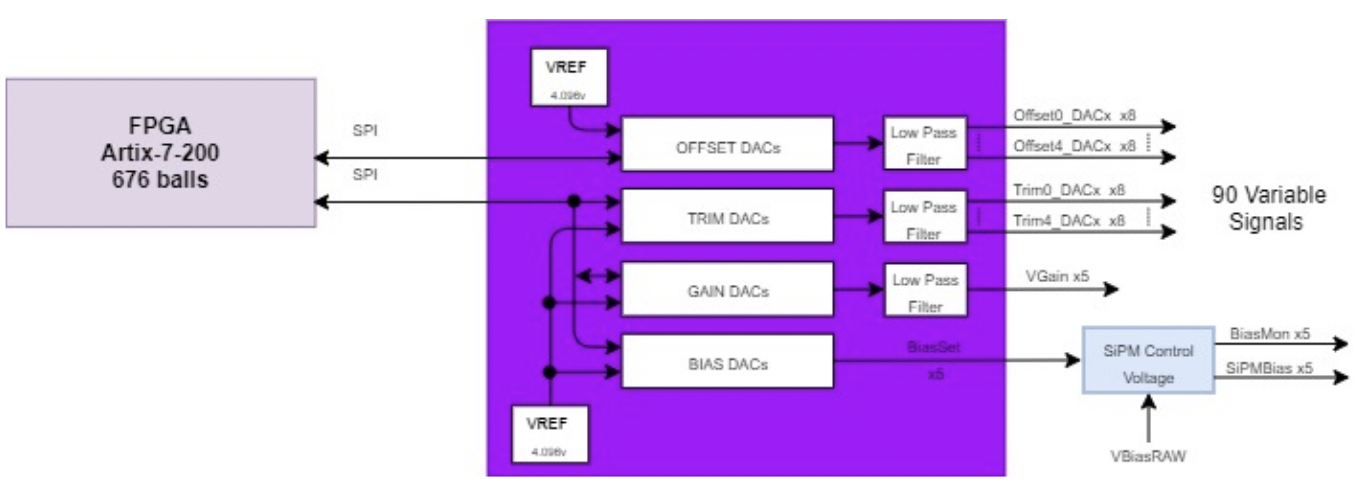
\includegraphics[width=.8\textwidth,trim=30 110 0 0,clip]{Images/BiasControl.png}
%\qquad
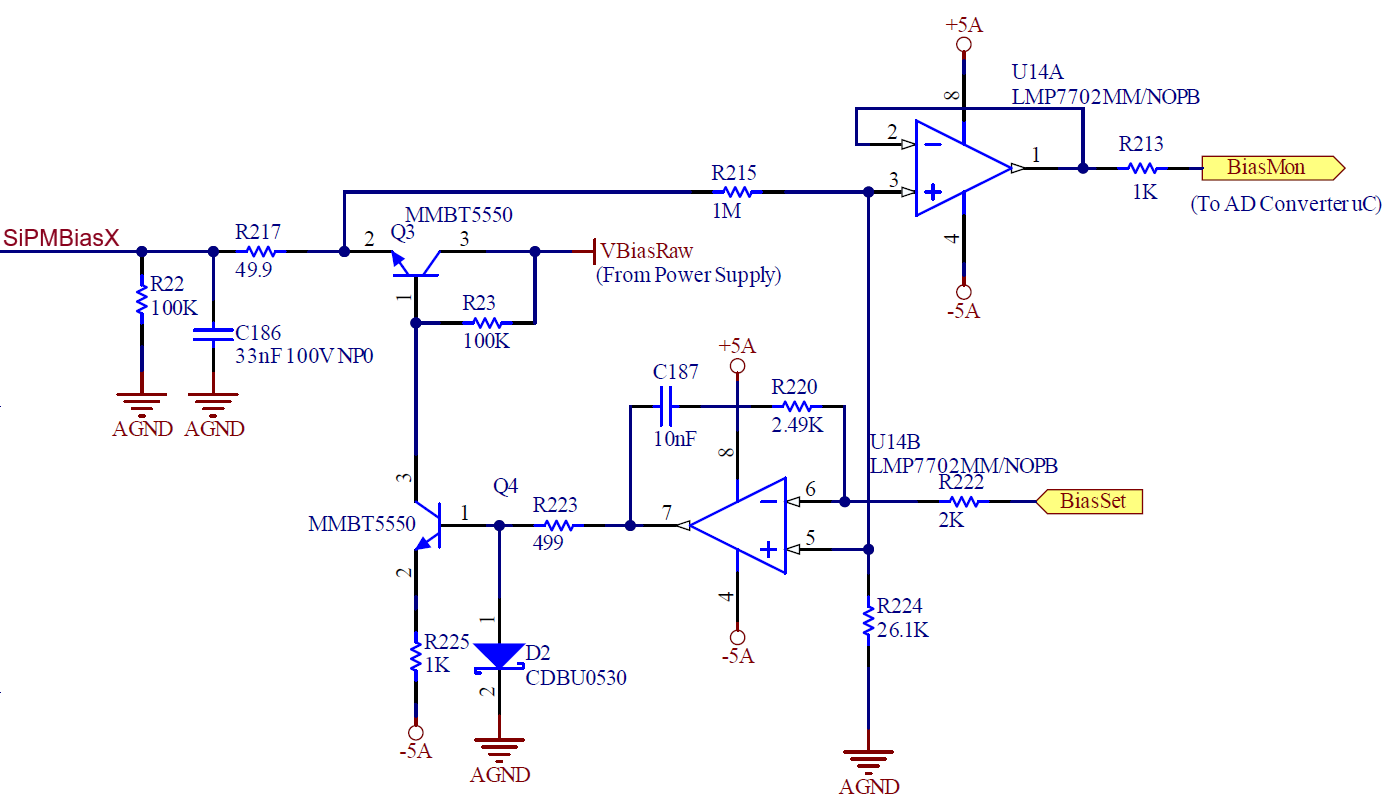
\includegraphics[width=.8\textwidth,origin=c,angle=0]{Images/BiasCircuit_v2.png}
% "\includegraphics" from the "graphicx" permits to crop (trim+clip)
% and rotate (angle) and image (and much more)
\caption{\label{fig:BiasCircuit} Bias voltage and monitoring circuit.}
\end{figure}

\subsubsection{Trimming voltage}

DAPHNE supports 40 trimming voltages, one for each channel. This voltage is variable from 0 to 4.096 V by using 5 AD5328 DAC devices. 

Figure~\ref{fig:TrimmCircuit} shows the different stages of one Trimming voltage generation, in this TRIM2\_DAC0. In this case, DAC2\_0 is a signal generated for the DAC, controlled by a SPI supported by the FPGA. Then, the signal is connected to a LMP7704 op-amp, to generate the TRIM2\_DAC0 signal. that is finally connected to the corresponding pin on the CE interface and to the monitoring interface.

\begin{figure}[htbp]
\centering % \begin{center}/\end{center} takes some additional vertical space
%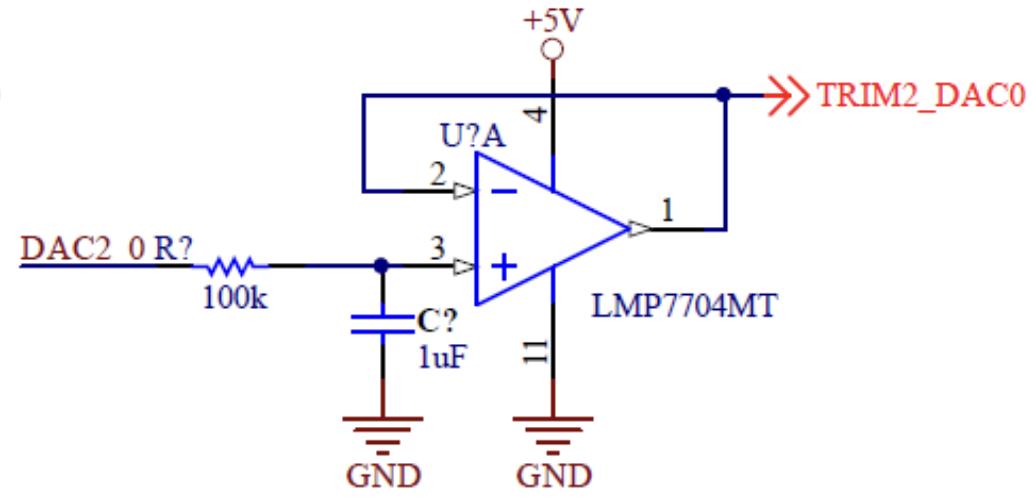
\includegraphics[width=.8\textwidth,trim=30 110 0 0,clip]{Images/TrimmCircuit.png}
%\qquad
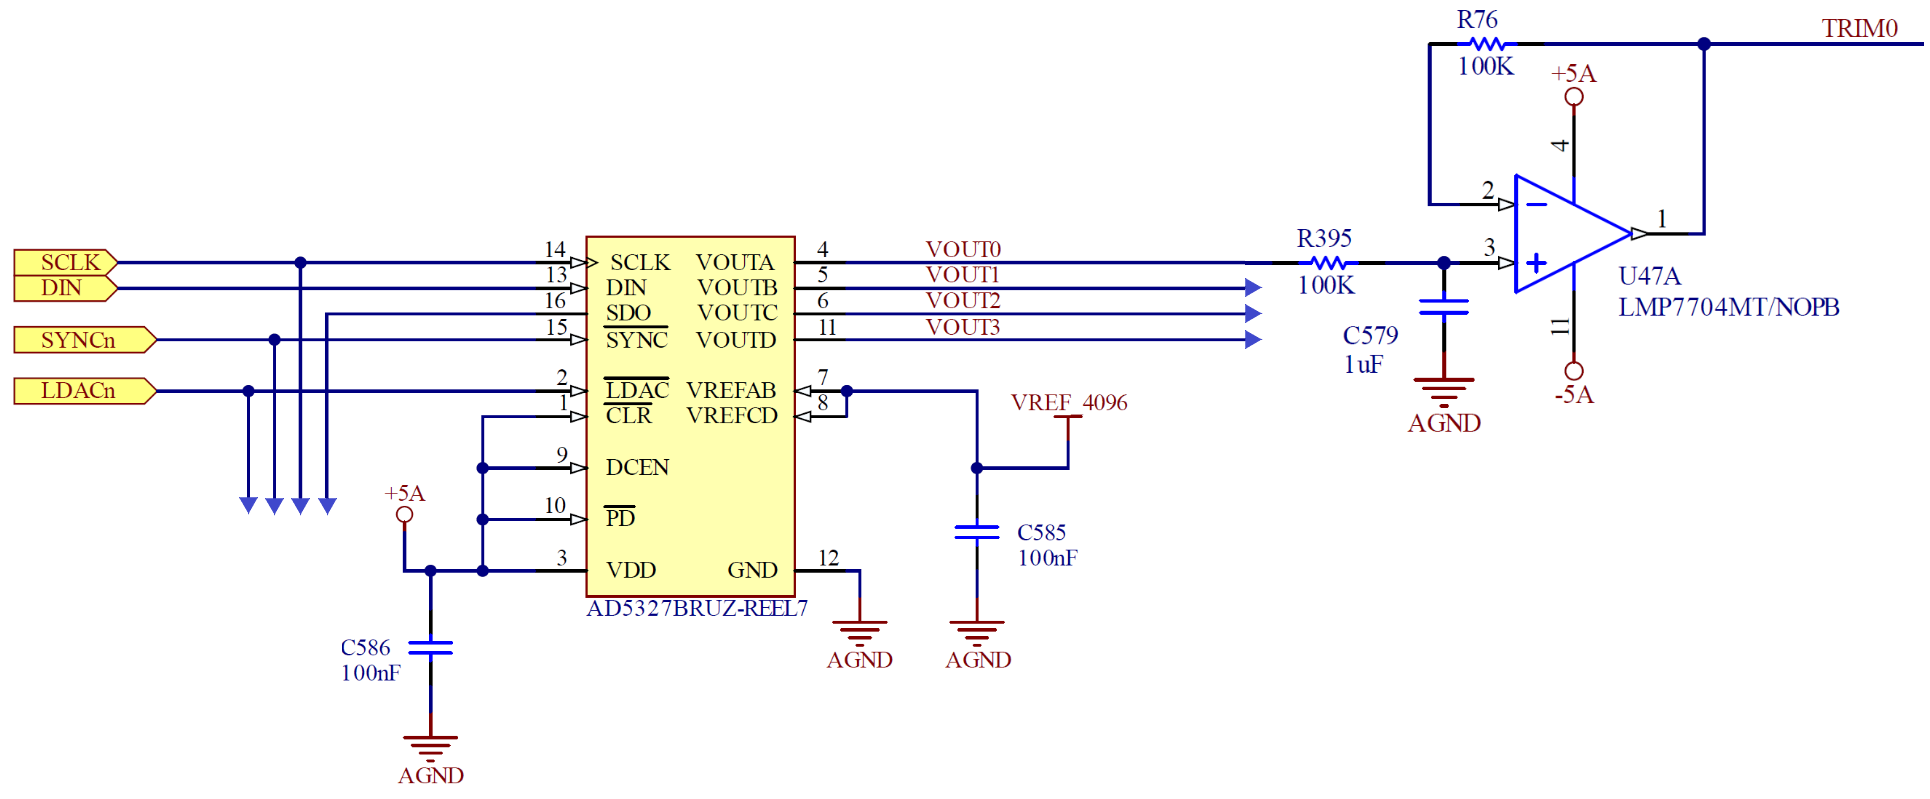
\includegraphics[width=.8\textwidth,origin=c,angle=0]{Images/TRIMCircuit_v2.png}
% "\includegraphics" from the "graphicx" permits to crop (trim+clip)
% and rotate (angle) and image (and much more)
\caption{\label{fig:TrimmCircuit} Trimming voltage generation circuit.}
\end{figure}

\subsubsection{Offset voltage}

An offset voltage is intended to generate a shift on the AFE input, required for analog to digital conversion. The scheme is the same as used for the trimming voltage, except that it does not use an op-amp stage to generate the signal after the DAC output.

The function of the offset voltage is shifting the signal to generate a behavior similar to a bipolar signal, but taking into account that the signal on the AFE input is unipolar, coming from the transformer that performs the differential to single conversion. This feature is one of the main differences between DAPHNE and the Mu2e board, because in the original design (Mu2e) the input is bipolar given the nature of the experiment and the AFE is configured to work with this kind of signals and in this case the by default configuration implies a DC-offset correction. 
If the PDS signals, that are unipolar are connected to the AFE in the same way of Mu2e, the result is that the analog conversion is performed only for the half of the range of the device and it is not effective to use a offset to force the AFE to convert in the entire range, because this offset would be eliminated for the DC-offset correction circuit.

During the DAPHNE design, it was found that it is possible disabling the DC-offset correction circuit, allowing the implementation of the offset shift for the unipolar signals and uses the AFE in the full conversion range in this way. 

\subsubsection{Cold electronics voltage}

 For the cold electronics voltage it used a +3V. To generate this voltage both a buck converter, LTC3624, and linear regulator, TPS7A701, are used. The buck converter will take +5.5V coming from the power transformer and convert it into +3.3V. The +3.3V will not be used for any other part of the board or FPGA. The linear regulator will then convert the voltage to +3V. Both the LTC3624 and TPS7A701 are adjustable so if a different cold electronics voltage was decided upon other than +3V then it could done by changing feed back resistors.

\subsubsection{Current and voltage monitoring}

DAPHNE is also responsible for the monitoring of currents and voltages delivered to each channel. There are 2 kind of signals to be monitored:

\begin{itemize}
  \item Voltages from the power supply
\item Bias and trimming voltage, with current monitoring
\end{itemize}
The monitoring is implemented by 2 separated ADCs with different resolutions:
\begin{itemize}
    \item Internal ADC on the STM32 microcontroller, which monitor Bias voltages (BiasMonX signals) and power supply voltages
\item ADC ADS1259, one-channel, delta-sigma, 24 bit, 14.4 Ksps for monitoring og trimming voltages %(DAx and DBx signals, referred to the figure 13)
\end{itemize}

In the case of the power supplies voltages, the interest is to have information about the state of the power supply and generates the corresponding alarms/flags, as well as initiate the required control actions in the case of an abnormal situation. Bias voltages are monitored with a low precision using the microcontroller ADC, taking into account that the bias generation is considered stable from the power supply. For the trimming voltage, it requires a better resolution for that reason DAPHNE has a high-resolution and high-performance ADC dedicated for this task. The implemented scheme to monitor the 40 trimming voltages includes a 2-stage analog-multiplexer based on ADG1609 IC and a single to differential conversion by using PGA280 amplifier, in order to generate the required differential signal for the ADS1259 ADC, as shown in figure~\ref{fig:CurrentandVoltageMonitoring}

\begin{figure}[htbp]
\centering % \begin{center}/\end{center} takes some additional vertical space
%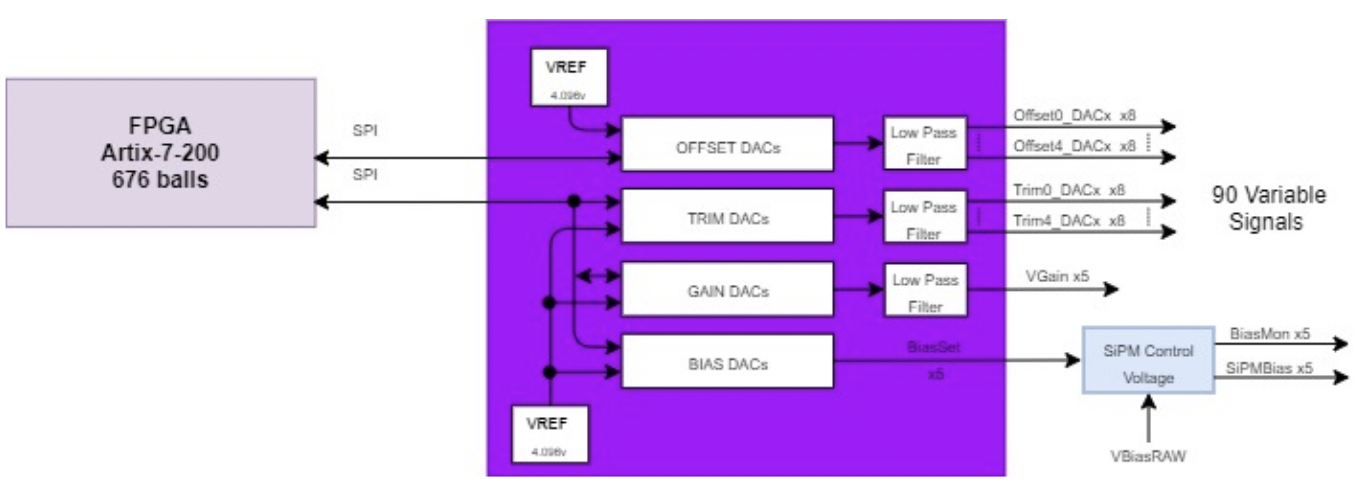
\includegraphics[width=.8\textwidth,trim=30 110 0 0,clip]{Images/BiasControl.png}
%\qquad
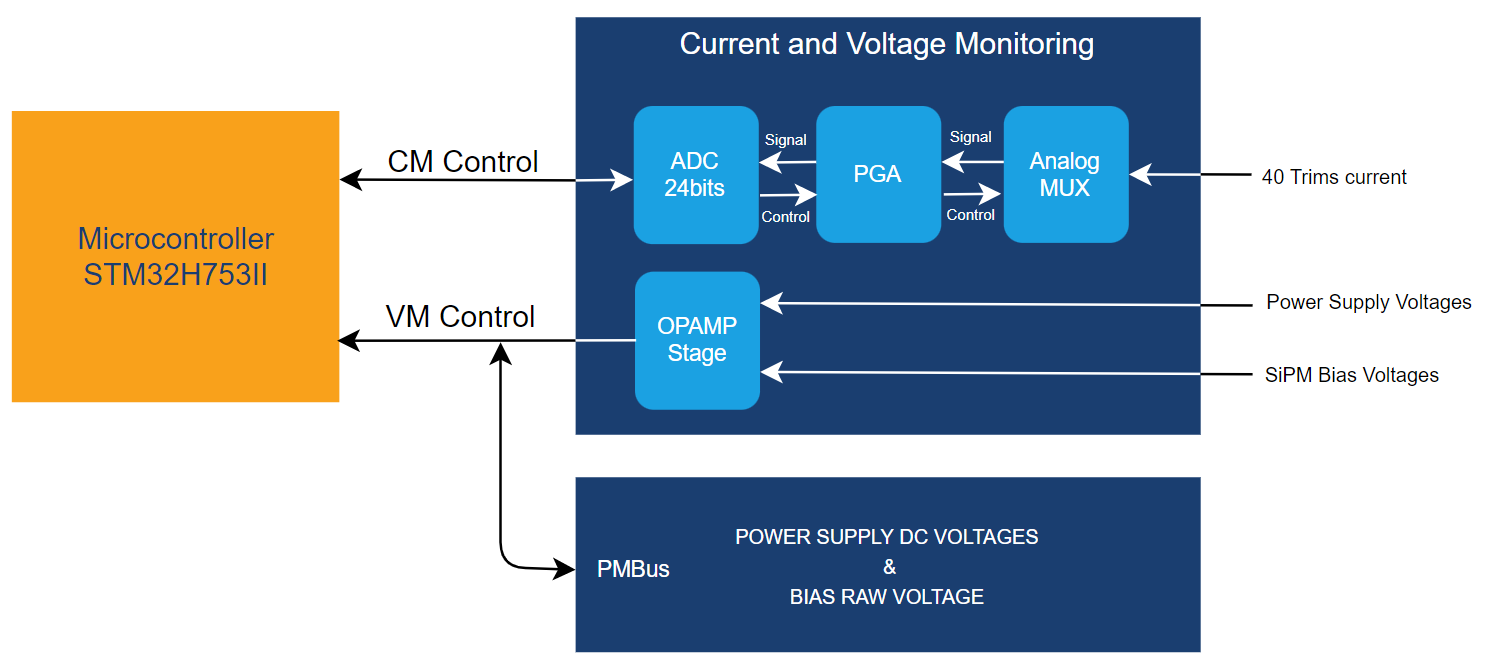
\includegraphics[width=.8\textwidth,origin=c,angle=0]{Images/CurrentandVoltageMonitoringV2.png}
% "\includegraphics" from the "graphicx" permits to crop (trim+clip)
% and rotate (angle) and image (and much more)
\caption{\label{fig:CurrentandVoltageMonitoring} Current and voltage monitoring.}
\end{figure}


%The digitization module consist of a differential to single converter, the AFE, and a readout control interface.  

\subsection{Slow control }

The main function of this interface is supporting slow control commands to be finally executed for the FPGA or the uC, depending on the peripherals to be controlled. The slow control consists of a fast ethernet connection controlled by the ST microcontroller, that uses a chain with a Wiznet chip and a PHY. The output of the link is a SFP transceiver, allowing optical fiber, RJ45 and a TCP/IP support.
The interface should handle flags in the power requirements of the board, allows monitoring of the XADCs on the FPGA and the General Error Handling of the FEB and Cold Electronics. 

The microcontroller communicates to the Wiznet via parallel interface, sending the required byte to be transmitted. The Wiznet supports the Fast Ethernet signaling and is connected to the PHY with optical fiber support. Finally, the PHY is connected to a SFP connector, intended to be used as a receptacle for specific transceivers, for example optical fiber or RJ-45. At the same time, there is a parallel interface connecting the FPGA and the microcontroller. The main source of data is the FPGA, that controls the data streaming from the AFE/ADC and eventually is necessary to communicate data through the Fast Ethernet Interface for debugging purposes. 

The FEB implements a server where a register matrix is refreshed in the microcontroller and in the FPGA. An error handling protocol is designed.

\subsection{DAQ}

One of the most important task that DAPHNE is required to accomplish is the communication of the signals generated by the PDS inside of the cryostat to the outside world. DAPHNE counts on two SFP transceivers for data streaming. This interface is supported by the GTP transceiver on the FPGA and are 6.6Gb/s capable in streaming mode. This special module allows DAPHNE to have a direct connection to an SFP connector. DAPHNE has 2 GTP connections, each one with a SFP connector including SFP cage, allowing the connection of any compatible SFP transceiver. In this case the purpose is connecting an optical fiber transceiver. Each SFP connector includes an I2C interface for control and configuration, connected to FPGA.

Both GTP Transceivers use a dedicated clock signal based on a crystal. The exact frequency of this crystal should be defined depending on the Full-mode specification and the adaptation to the half of the maximum rate proposed to operate on DAPHNE. The operation of this interface depends on the digital module implemented on the FPGA.

\subsection{Timing Recovery CDR}
The DAPHNE CDR module is based on the SoLiD CDR module developed at the University of Bristol~\cite{Arnold_2017}. The DUNE DAQ system provides a system clock of 62.5MHz for DAPHNE that is connected at the CDR port (Optical fiber). The module has an SFP connector for optical fiber support by using a transceiver. The signal is connected to an ADC2814 Clock and data recovery chip, which provides 2 separated data and clock signal. The data signal is connected to the FPGA in order to be used in the appropriate modules. The SFP connection has a dedicated i2c interface connected to the FPGA, used to control and monitor the interface.

The recovered clock signal is connected to a clock generator block, which includes a PLL, a low-pass filter, and a controlled oscillator. This block generates a continuous  clock signal depending on the Timing Interface input and the clock generator. The design includes the capability of continuing working even if the Timing Interface is disconnected. The CDR chip can detect the loss of the external signal and there is a flag for the control module. 

\subsection{LEMO connectors}

DAPHNE has 2 LEMO connectors intended to be used as external triggering and timing signals, in this case 1 input and 1 output. These connectors are directly connected clock capable pins on the FPGA and should be included in the gate structure implemented on the Artix-7.


\subsubsection{LEMO input} DAPHNE is prepared to work with an external clock input source at the LEMO connection. This connection will be used during the tests in absence of a system triggering clock, or with different rates at the streaming output.

\subsubsection{LEMO output}
The LEMO output allows us to sync other modules sharing the clock of the FPGA. It could be the LEMO input clock or the one of the inner programmable clock on the FPGA. A control loop can be runned to check the clock integrity of some modules or signals